\newpage
\section{QR decomposition}
\label{sec:QR}



%%%%%%%%%%%%%%%%%%%%%%%%%%%%%%%%%%%%%%%%%%%%%%%%%%%%%%%%%%%%%%%%%%%%%%%%%%%%%%%%%%%%%%%%%%%%%%%%%%%%
\subsection{Theory}
%%%%%%%%%%%%%%%%%%%%%%%%%%%%%%%%%%%%%%%%%%%%%%%%%%%%%%%%%%%%%%%%%%%%%%%%%%%%%%%%%%%%%%%%%%%%%%%%%%%%



%%%%%%%%%%%%%%%%%%%%%%%%%%%%%%%%%%%%%%%%%%%%%%%%%%

\subsubsection{Orthogonal matrices}
\label{sec:orthogonalMatrices}

Orthogonal matrices represent either reflections or rotations and fulfill by definition the equations:

\begin{align}
\label{eq:definitionOrthogonal0}
\mathbf{Q}\mathbf{Q}^T = \mathbf{I}\\
\label{eq:definitionOrthogonal1}
\mathbf{Q}^T\mathbf{Q} = \mathbf{I}
\end{align}
%
Therefore, the transposed of an orthogonal matrix is also its inverse:
\begin{align}
\label{eq:orthogonalInverse}
\mathbf{Q}^T = \mathbf{Q}^{-1}
\end{align}
%
Another useful property of orthogonal matrices is, that they preserve the length of a vector during matrix-vector multiplication:
\begin{align}
\label{eq:orthogonalPreserveLength}
\norm{\mathbf{Qx}}= \norm{\mathbf{y}}
\end{align}



%%%%%%%%%%%%%%%%%%%%%%%%%%%%%%%%%%%%%%%%%%%%%%%%%%

\subsubsection{Solving linear systems with QR decomposition}

QR decomposition decomposes a matrix $\mathbf{A}$ into an orthogonal matrix $\mathbf{Q}$ and an upper triangular matrix $\mathbf{R}$. 
Solving linear systems with QR decomposition is pretty much straight forward:
\begin{align}
\mathbf{A}\mathbf{x} &= \mathbf{r}\\
\mathbf{QR}\mathbf{x} &= \mathbf{r}
\end{align}
%
The product $\mathbf{R}\mathbf{x}$ is substituted by the vector $\mathbf{y}$:

\begin{align}
\mathbf{Qy} &= \mathbf{r}
\end{align}
%
Since $\mathbf{Q}$ is orthogonal, it follows:

\begin{align}
\mathbf{y} &= \mathbf{Q}^{-1}\mathbf{r}\\
\label{eq:qrSolveIntermediate}
\mathbf{y} &= \mathbf{Q}^T\mathbf{r}
\end{align}
%
The system's solution $\mathbf{x}$ is now obtained by simple backward substitution (see \cref{sec:backwardSubstitution}) because of $\mathbf{R}$ being an upper triangular matrix.
\begin{align}
\mathbf{R}\mathbf{x} = \mathbf{y}
\end{align}
%
The QR decomposition itself can be calculated with different techniques, namely the Gram-Schmidt process, Givens rotations and Householder reflections.
In this document, Householder reflections are used to calculate the decomposition.
In contrast to the Gram-Schmidt approach, they produce numerically stable results.
Their disadvantage of not being parallelizable is not relevant, since systems which benefit of parallelization are usually to large for a real-time engine.
Givens rotations are much more complex regarding the implementation without offering any real benefit within the scope of small linear systems. 
 


%%%%%%%%%%%%%%%%%%%%%%%%%%%%%%%%%%%%%%%%%%%%%%%%%%

\subsubsection{Householder reflections}

A householder reflection is a reflection at a plane or hyperplane that contains the origin of the coordinate system.
Because the origin is by definition part of the reflection plane, only its normal $\mathbf{w}$ is needed to describe it mathematically.
An example is shown in \cref{fig:housholderReflection}.
The Householder matrix $\mathbf{H}$ which performs the reflection can be calculated as follows:


\begin{figure}
	\centering
	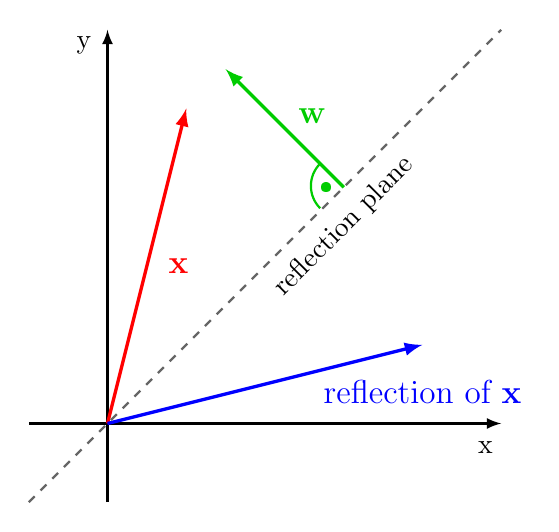
\begin{tikzpicture}
	\draw[color=black,-latex,thick] (-1,0)--(5,0);
	\draw[color=black,-latex,thick] (0,-1)--(0,5);
	\draw[color=red,-latex,very thick] (0,0)--(1,4);
	\draw[color=blue,-latex,very thick] (0,0)--(4,1);
	\draw[color={black!20!green},-latex,very thick] (3,3)--(1.5,4.5);
	\draw[color={black!20!green}, thick] (2.7,3.3) arc (135:225:0.4);
	\node[color={black!20!green}] at (2.78,2.98) {\textbullet};
	\draw[color={black!60!white},dashed,thick] (-1,-1)--(5,5);
	\node[] at (4.8,-0.3) {x};
	\node[] at (-0.3,4.8) {y};
	\node[color=red] at (0.9,2) {\large{$\mathbf{x}$}};
	\node[color=blue] at (4,0.4) {\large{reflection of $\mathbf{x}$}};
	\node[color={black!20!green}] at (2.6,3.9) {\large{$\mathbf{w}$}};
	\node[rotate=45] at (3,2.5) {reflection plane};
	\end{tikzpicture}
	\caption{Householder reflection}
	\label{fig:housholderReflection}
\end{figure}


\begin{align}
\label{eq:householderGeneral}
\mathbf{H} = \mathbf{I} - \frac{2}{\mathbf{w}^T\mathbf{w}}\mathbf{w}\mathbf{w}^T
\end{align}
%
$\mathbf{w}^T\mathbf{w}$ is the scalar product. With $\mathbf{v}$ being the unit normal of the reflection plane

\begin{align}
	\mathbf{v} = \frac{1}{\norm{\mathbf{w}}}\mathbf{w}
\end{align}
%
\cref{eq:householderGeneral} simplifies to:

\begin{align}
\label{eq:householderUnitLength}
\mathbf{H} = \mathbf{I} - 2\mathbf{v}\mathbf{v}^T
\end{align}
%
The Householder matrix $\mathbf{H}$ has some useful properties.
First, it is orthogonal (\cref{sec:orthogonalMatrices}).
Additionally, it is also symmetric, meaning:

\begin{align}
\label{eq:householderSymmetric}
\mathbf{H} = \mathbf{H}^T
\end{align}
%
Combining \cref{eq:householderSymmetric} with \cref{eq:orthogonalInverse} yields:

\begin{align}
\label{eq:householderInverse}
\mathbf{H} = \mathbf{H}^{-1}
\end{align}
%
So a Householder matrix is its own inverse.
Furthermore, abusing the Householder matrix's special structure, the product with another vector or matrix can be computed more efficiently than the standard matrix-vector product or matrix-matrix product:

\begin{align}
\nonumber
\mathbf{H} \mathbf{x}
&= 
\pth{\mathbf{I} - 2\mathbf{v}\mathbf{v}^T}\mathbf{x}
\\&= 
\nonumber
\mathbf{I}\mathbf{x} - 2\mathbf{v}\mathbf{v}^T\mathbf{x}
\\&= 
\label{eq:householderEfficientMatrixVector}
\mathbf{x} - 2\pth{\mathbf{v}^T\mathbf{x}}\mathbf{v}
\end{align}
%
Note that $\mathbf{v}^T\mathbf{x}$ is the scalar product.
Instead of the quadratic complexity of the standard matrix-vector product, \cref{eq:householderEfficientMatrixVector} is only of linear complexity.
For matrix-matrix multiplication the approach is similar and results in quadratic complexity instead of cubic:

\begin{align}
\label{eq:householderEfficientMatrixMatrix}
\mathbf{H} \mathbf{A}
=
\mathbf{A} - 2\mathbf{v}\pth{\mathbf{v}^T\mathbf{A}}
\end{align}
%
$\mathbf{v}^T\mathbf{A}$ is a row vector that contains the scalar products of $\mathbf{v}$ and each column of $\mathbf{A}$



%%%%%%%%%%%%%%%%%%%%%%%%%%%%%%%%%%%%%%%%%%%%%%%%%%

\subsubsection{Calculation of a specific Householder reflection}
\label{sec:householderCalculateSpecificReflection}

Consider the case, that two vectors $\mathbf{x}$ and $\mathbf{y}$ of arbitrary length are known and the reflection, which transforms $\mathbf{x}$ in a way that it points into the same direction as $\mathbf{y}$, should be determined.
The equation that describes this problem is:

\begin{align}
\label{eq:housholderCalculateReflection}
\mathbf{H} \mathbf{x} = \lambda \mathbf{y}
\end{align}
%
Since orthogonal matrices preserve a vectors length (see \cref{eq:orthogonalPreserveLength}) it follows:

\begin{align}
\label{eq:housholderCalculateReflectionLambda}
\lambda = \pm \frac{\norm{\mathbf{x}}}{\norm{\mathbf{y}}}
\end{align}
%
So $\lambda$ is the length ratio of the vectors $\mathbf{x}$ and $\mathbf{y}$.
Taking a look at \cref{fig:housholderCalculateReflection} reveals that the difference between the vectors $\mathbf{x}$ and $\mathbf{Hx}$ is orthogonal to the reflection plane.
Therefore, it is a normal of this plane.
Hence, the vector $\mathbf{v}$ of the required Householder reflection can be calculated with:

\begin{align}
\label{eq:housholderCalculateReflectionNormal}
\mathbf{v} = \frac{\mathbf{x} - \lambda \mathbf{y}}{\norm{\mathbf{x} - \lambda \mathbf{y}}}
\end{align}


\begin{figure}
\centering
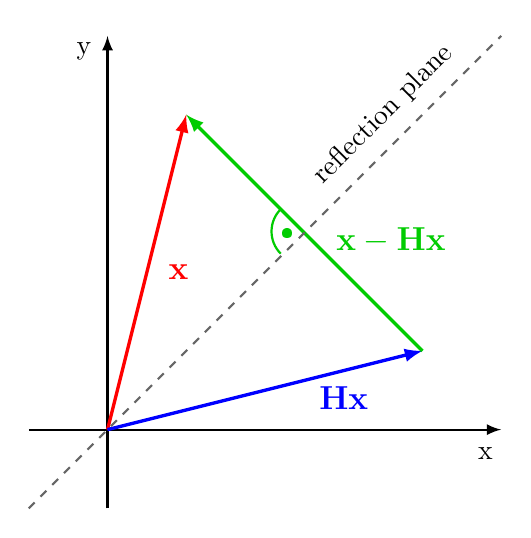
\begin{tikzpicture}
\draw[color=black,-latex,thick] (-1,0)--(5,0);
\draw[color=black,-latex,thick] (0,-1)--(0,5);
\draw[color=red,-latex,very thick] (0,0)--(1,4);
\draw[color=blue,-latex,very thick] (0,0)--(4,1);
\draw[color={black!20!green},-latex,very thick] (4,1)--(1,4);
\draw[color={black!20!green}, thick] (2.2,2.8) arc (135:225:0.4);
\node[color={black!20!green}] at (2.28,2.48) {\textbullet};
\draw[color={black!60!white},dashed,thick] (-1,-1)--(5,5);
\node[] at (4.8,-0.3) {x};
\node[] at (-0.3,4.8) {y};
\node[color=red] at (0.9,2) {\large{$\mathbf{x}$}};
\node[color=blue] at (3,0.4) {\large{$\mathbf{Hx}$}};
\node[color={black!20!green}] at (3.6,2.4) {\large{$\mathbf{x-Hx}$}};
\node[rotate=45] at (3.5,4) {reflection plane};
\end{tikzpicture}
\caption{Difference between original and reflected vector}
\label{fig:housholderCalculateReflection}
\end{figure}



%%%%%%%%%%%%%%%%%%%%%%%%%%%%%%%%%%%%%%%%%%%%%%%%%%

\subsubsection{Calculation of the decomposition}

\draftNote{
\begin{itemize}
\item Update with 4x4 matrix
\item Use bars instead of superscripts to differ between intermediate results 
\end{itemize}	
}

The algorithm to calculate the QR decomposition using Householder reflections is not too hard to understand once you understood the concepts of the previous sections.
A series of Householder reflections is calculated and multiplied with the target matrix, so that each value below the main diagonal becomes 0.
At the end of this process, the upper triangular matrix $\mathbf{R}$ is obtained.
The matrix $\mathbf{Q}$ can be calculated by multiplication of all used Householder reflection, but usually, it is not necessary to calculate it explicitly.
The procedure is discussed on a small example.
Consider the linear System $\mathbf{Ax} = \mathbf{r}$ with:

\begin{align*}
\mathbf{A}
=
\begin{bmatrix}
a_0&b_0&c_0\\
a_1&b_1&c_1\\
a_2&b_2&c_2
\end{bmatrix}
&&
\mathbf{x}
=
\begin{bmatrix}
x_0\\
x_1\\
x_2
\end{bmatrix}
&&
\mathbf{r}
=
\begin{bmatrix}
r_0\\
r_1\\
r_2
\end{bmatrix}
\end{align*}

The algorithm starts by calculating a Householder reflection that turns all values of the first column below the main diagonal into zeros:

\begin{align}
\mathbf{H}_0\mathbf{A} 
=
\mathbf{A}_1
=
\begin{bmatrix}
a_0^1&b_0^1&c_0^1\\
0    &b_1^1&c_1^1\\
0    &b_2^1&c_2^1
\end{bmatrix}					  
\end{align}
%
Note that the superscripted numbers are just used to differ between members of $\mathbf{A}$ and $\mathbf{A}_1$ and shouldn't be understood as mathematical exponent.
The necessary transformation must reflects the first column of $\mathbf{A}$, which will be denoted as $\mathbf{a}$, onto the axis
\begin{align}
\mathbf{e}_0  
=
\begin{bmatrix}
1\\
0\\
0
\end{bmatrix}
\end{align}
%
Using \cref{eq:housholderCalculateReflectionNormal} yields

\begin{align}
\mathbf{v}_0 
&= 
\frac{1}{\norm{\mathbf{a} - \lambda_0 \mathbf{e}_0}}\pth{\mathbf{a} - \lambda_0 \mathbf{e}_0}\\
&=
\frac{1}{\norm{\mathbf{a} - \lambda_0 \mathbf{e}_0}}
\pth{
\begin{bmatrix}
a_0\\
a_1\\
a_2
\end{bmatrix}
-	
\lambda_0	
\begin{bmatrix}
1\\
0\\
0
\end{bmatrix}
}\\
\label{eq:qrReflectionVector0StillContainingLambda}
&=
\frac{1}{\norm{\mathbf{a} - \lambda_0 \mathbf{e}_0}}
\begin{bmatrix}
a_0 - \lambda_0\\
a_1\\
a_2
\end{bmatrix}
\end{align}
%
Since $\mathbf{e}_0$ is of unit length, \cref{eq:housholderCalculateReflectionLambda} gives:

\begin{align}
\lambda_0 = \pm \norm{\mathbf{a}}
\end{align}
%
Generally, the sign can be chosen freely, but for numerical reasons one should pick the opposite sign of $a_0$. 
This way the result with the larger magnitude is selected from $a_0 -  \pm \norm{\mathbf{a}}$.
To illustrate why this is necessary, consider the case $\mathbf{a} = \mathbf{e}_0$.
Using the same sign yields:

\begin{align}
\mathbf{e}_0 - \norm{\mathbf{e}_0}\mathbf{e}_0 
=
\begin{bmatrix}
1 - \norm{\mathbf{e}_0}\\
0\\
0
\end{bmatrix}
=
\begin{bmatrix}
0\\
0\\
0 
\end{bmatrix}
\end{align}
%
and in result:

\begin{align}
\frac{1}{\norm{\mathbf{e}_0 - \norm{\mathbf{e}_0}\mathbf{e}_0}} = \frac{1}{\color{red}{\mathbf{0}}}
\end{align}
%
Choosing the opposite sign prevents this from happening unless $\mathbf{a}$ is already of length 0, which would indicate that the matrix is singular.
Combining 


\begin{align}
\lambda_0 = -\textrm{sign}\pth{a_0} \norm{\mathbf{a}}
\end{align}
%
with \cref{eq:qrReflectionVector0StillContainingLambda} yields:



\begin{align}
\mathbf{v}_0 
&=
\frac{1}{\norm{\mathbf{w}_0}}\mathbf{w}_0
\end{align}
%
with:

\begin{align}
\mathbf{w}_0 
&=
\begin{bmatrix}
a_0 + \textrm{sign}\pth{a_0} \norm{\mathbf{a}}\\
a_1\\
a_2
\end{bmatrix}
\end{align}
%
Now the intermediate matrix $\mathbf{A}_1$ can be determined by calculating $\mathbf{H}_0$ ( \cref{eq:householderUnitLength}) and applying it to $\mathbf{A}$.
However, the more efficient way is to use \cref{eq:householderEfficientMatrixMatrix}.

After obtaining $\mathbf{A}_1$, another reflection $\mathbf{H}_1$ is calculated which turns every value of the second column that is located below the main diagonal into zeros:

\begin{align}
\mathbf{H}_1\mathbf{H}_0\mathbf{A} 
= 
\mathbf{H}_1\mathbf{A}_1
= 
\mathbf{A}_2
=
\begin{bmatrix}
a_0^2&b_0^2&c_0^2\\
0    &b_1^2&c_1^2\\
0    &0    &c_2^2
\end{bmatrix}					  
\end{align}
%
Note that $\mathbf{H}_1$ must be constructed in a way, that it doesn't affect values that lie on the axis $\mathbf{e}_0$ (first row of $\mathbf{A}_1$).
Otherwise, because of \cref{eq:orthogonalPreserveLength}, one or more values below $a_0^1$ in the first column of $\mathbf{A}_1$ will become different from 0 again.
This means that the reflection plane must contain the axis $\mathbf{e}_0$.
Hence, the reflection plane's normal $\mathbf{v}_1$ must have the form: 

\begin{align}
\label{eq:qrReflectionVector1Requirement}
\mathbf{v}_1
= 
\begin{bmatrix}
0\\
v_1^1\\
v_2^1
\end{bmatrix}
\end{align}
%
The corresponding Householder matrix $\mathbf{H}_1$ would be (\cref{eq:householderUnitLength}):

\begin{align}
\mathbf{H}_1
=
\begin{bmatrix}
1    &0            &0       \\
0    &1- v_1^1v_1^1&  v_2^1v_1^1\\
0    &   v_1^1v_2^1&1-v_2^1v_2^1
\end{bmatrix}					  
\end{align}
%
Since the values on the axis $\mathbf{e}_0$ should remain constant, it is sufficient to continue working with a reduced system by removing the corresponding rows and columns:

\begin{align}
\mathbf{\hat{A}}_1
=
\begin{bmatrix}
b_1^1&c_1^1\\
b_2^1&c_2^1
\end{bmatrix}					  
\end{align}


\begin{align}
\mathbf{\hat{H}}_1\mathbf{\hat{A}}_1
= 
\mathbf{\hat{A}}_2
=
\begin{bmatrix}
b_1^2&c_1^2\\
0    &c_2^2
\end{bmatrix}					  
\end{align}
%
Now the calculation of the reflection can be performed exactly as during the first step, yielding the vector 

\begin{align}
\mathbf{\hat{v}}_1
=
\begin{bmatrix}
v_1^1\\
v_2^1
\end{bmatrix}
\end{align}
%
which is the reduced equivalent of $\mathbf{v}_1$ (compare with \cref{eq:qrReflectionVector1Requirement}).
At this point, the decomposition process is finished, because $\mathbf{A}_2$ is already an upper triangular matrix.

\begin{align}
\mathbf{A}_2 = \mathbf{R}
\end{align}
%
For larger matrices the algorithm would simply continue column by column until $\mathbf{R}$ is obtained.
Because of 

\begin{align}
\mathbf{R} = \mathbf{H}_1\mathbf{H}_0\mathbf{A} = \mathbf{Q}^T\mathbf{A}
\end{align}
%
it follows: 

\begin{align}
\mathbf{Q}^T &= \mathbf{H}_1\mathbf{H}_0\\
\nonumber
\mathbf{Q}   &= \pth{\mathbf{H}_1\mathbf{H}_0}^T\\
\nonumber
&= \mathbf{H}_0^T\mathbf{H}_1^T\\
&= \mathbf{H}_0\mathbf{H}_1
\end{align}
%
However, calculating $\mathbf{Q}$ is usually expensive and not necessary. Instead, the reflection normals $\mathbf{v}_0$ and $\mathbf{v}_1$ are stored and used during the solution process, taking advantage of the effective matrix-vector and matrix-matrix products (\cref{eq:householderEfficientMatrixMatrix,eq:householderEfficientMatrixVector}).
So instead of using \cref{eq:qrSolveIntermediate}, the intermediate result $\mathbf{y}$ is calculated with:

\begin{align}
\mathbf{y} &= \mathbf{H}_1\mathbf{H}_0\mathbf{r}
\end{align}
%



%%%%%%%%%%%%%%%%%%%%%%%%%%%%%%%%%%%%%%%%%%%%%%%%%%

\subsubsection{Algorithm summary}

This section is just a short summary of the algorithm presented in the previous sections.
They should be read first.

For an arbitrary matrix $\mathbf{A}$ of size $N \times N$ calculate:

\begin{align}
\label{eq:qrReflectionUnitNormal}
\mathbf{v} 
&=
\frac{1}{\norm{\mathbf{w}}}\mathbf{w}
\end{align}
%
with 

\begin{align}
\label{eq:qrReflectionNormal}
\mathbf{w} = 
\begin{bmatrix}
a_{00} + \textrm{sign}\pth{a_{00}} \norm{\mathbf{a}_1}\\
a_{10}\\
\vdots\\
a_{\pth{N-1}0}
\end{bmatrix}
\end{align}
%
The vector $\mathbf{a}_1$ is the first column of $\mathbf{A}$. 
Use \cref{eq:householderEfficientMatrixMatrix} to obtain the result of

\begin{align}
\mathbf{H}_1 \mathbf{A} = \mathbf{A}_1
\end{align}
%
without calculating $\mathbf{H}_1$ explicitly.
Remove the first column and row of $\mathbf{A}_1$ and repeat this procedure with the reduced system until the upper triangular matrix $\mathbf{R}$ is obtained.
This will need $N-1$ Householder reflections.
Store the reflection normals $\mathbf{v}_1$ to $\mathbf{v}_{N-1}$ and the matrix $\mathbf{R}$ as QR factorization of $\mathbf{A}$.
To solve the system $\mathbf{A}\mathbf{x}=\mathbf{r}$, calculate the result of

\begin{align}
\mathbf{y} &= \mathbf{Q}^T\mathbf{r}\\
\mathbf{y} &= \mathbf{H}_{N-1} \hdots \mathbf{H}_{2}\mathbf{H}_{1}\mathbf{r}
\end{align}
%
using the vectors $\mathbf{v}_1$ to $\mathbf{v}_{N-1}$ and \cref{eq:householderEfficientMatrixVector}.
Finally, use backward substitution to obtain the systems result $\mathbf{x}$ from 

\begin{align}
\mathbf{R}\mathbf{x} &= \mathbf{y}
\end{align}




%%%%%%%%%%%%%%%%%%%%%%%%%%%%%%%%%%%%%%%%%%%%%%%%%%

\subsubsection{Rectangular matrices}

\draftNote{Start section}



%%%%%%%%%%%%%%%%%%%%%%%%%%%%%%%%%%%%%%%%%%%%%%%%%%%%%%%%%%%%%%%%%%%%%%%%%%%%%%%%%%%%%%%%%%%%%%%%%%%%
\subsection{Optimizations}
%%%%%%%%%%%%%%%%%%%%%%%%%%%%%%%%%%%%%%%%%%%%%%%%%%%%%%%%%%%%%%%%%%%%%%%%%%%%%%%%%%%%%%%%%%%%%%%%%%%%
\label{sec:qrOptimizations}



%%%%%%%%%%%%%%%%%%%%%%%%%%%%%%%%%%%%%%%%%%%%%%%%%%

\subsubsection{Calculation of vector norms}
\label{sec:qrOptimizationsVectorNorms}

During the calculation of each reflection's unit normal $\mathbf{v}$, two vector norms have to be calculated.
Both vectors only differ in a single value.
Therefore, the squared sum of all shared values needs to be calculated only once.

To illustrate this, have a look at the \cref{eq:qrReflectionNormal,eq:qrReflectionUnitNormal}.
In the vectors $\mathbf{a}_1$ and $\mathbf{v}$ share the values $a_{12}$ to $a_{1N}$.
With the sum 

\begin{align}
s =  \pth{a_{12}}^2  + \pth{a_{13}}^2 + \hdots + \pth{a_{1N}}^2  
\end{align}
%
the norms can be calculated as follows:

\begin{align}
\norm{\mathbf{a}_1} &= \sqrt{\pth{a_{11}}^2 + s}\\
\norm{\mathbf{w}} &= \sqrt{\pth{a_{11} + \textrm{sign}\pth{a_{11}} \norm{\mathbf{a}_1}}^2 + s}
\end{align}



%%%%%%%%%%%%%%%%%%%%%%%%%%%%%%%%%%%%%%%%%%%%%%%%%%

\subsection{Calculation of intermediate matrix}
\label{sec:qrOptimizationsFirstColumn}

At the end of each factorization step, a new intermediate matrix is calculated by using \cref{eq:householderEfficientMatrixMatrix}.
The applied reflection is constructed in a way that the first column of the resulting matrix contains only zeros below the first value.
Because orthogonal matrices preserve vector lengths (\cref{eq:orthogonalPreserveLength}), the only value of the resulting column that is not equal to zero, must be equal to the columns norm before the transformation.
This value was already determined during the reflection normal's calculation.
Hence, no further computations are needed to obtain the first column of the resulting matrix.



%%%%%%%%%%%%%%%%%%%%%%%%%%%%%%%%%%%%%%%%%%%%%%%%%%

\subsubsection{Compact factorization data storage}
\label{sec:qrOptimizationsCompactData}

At this point, it should be mentioned that storing the calculated reflection's unit normals instead of calculating Q explicitly is already an optimization regarding performance and memory consumption.
Storing all necessary unit normals column by column produces an $N \times \pth{N-1}$ matrix $\mathbf{V}$ with all values above the main diagonal being zeros.

\begin{align}
\mathbf{V} = 
\begin{bmatrix}
v_0 & 0         & 0\\
v_1 & \bar{v}_1 & 0\\
v_2 & \bar{v}_2 & \bar{\bar{v}}_2 \\
v_3 & \bar{v}_3 & \bar{\bar{v}}_3 \\
\end{bmatrix}
\end{align}
%
Its data can be stored together with the data of the upper triangular matrix $\mathbf{R}$ in the compact from:

\begin{align}
\mathbf{F} = 
\begin{bmatrix}
	v_0 & r_{00}    & r_{01}          & r_{02} & r_{03} \\
	v_1 & \bar{v}_1 & r_{11}          & r_{12} & r_{13} \\
	v_2 & \bar{v}_2 & \bar{\bar{v}}_2 & r_{22} & r_{23} \\
	v_3 & \bar{v}_3 & \bar{\bar{v}}_3 & -      & r_{33} \\
\end{bmatrix}
\end{align}




%%%%%%%%%%%%%%%%%%%%%%%%%%%%%%%%%%%%%%%%%%%%%%%%%%%%%%%%%%%%%%%%%%%%%%%%%%%%%%%%%%%%%%%%%%%%%%%%%%%%
\subsection{Implementation}
%%%%%%%%%%%%%%%%%%%%%%%%%%%%%%%%%%%%%%%%%%%%%%%%%%%%%%%%%%%%%%%%%%%%%%%%%%%%%%%%%%%%%%%%%%%%%%%%%%%%




%%%%%%%%%%%%%%%%%%%%%%%%%%%%%%%%%%%%%%%%%%%%%%%%%%%%%%%%%%%%%%%%%%%%%%%%%%%%%%%%%%%%%%%%%%%%%%%%%%%%
\newpage
\subsubsection{Solver for arbitrary sized matrices - Serial}




%%%%%%%%%%%%%%%%%%%%%%%%%%%%%%%%%%%%%%%%%%%%%%%%%%%%%%%%%%%%%%%%%%%%%%%%%%%%%%%%%%%%%%%%%%%%%%%%%%%%
\newpage
\subsubsection{Solver for arbitrary sized matrices - SIMD}

\draftNote{
	\begin{itemize}
		\item Remember that the calculation of multiple scalar products (calculation of $\mathbf{v}^T\mathbf{A}$) can be vectorized
	\end{itemize}
}